\documentclass[11pt, oneside]{article} 
\usepackage{geometry}
\geometry{letterpaper} 
\usepackage{graphicx}
	
\usepackage{amssymb}
\usepackage{amsmath}
\usepackage{parskip}
\usepackage{color}
\usepackage{hyperref}

\graphicspath{{/Users/telliott/Dropbox/Github-Math/geoproof/figures/}{/Users/telliott/Dropbox/Github-Math/figures/}}
% \begin{center} \includegraphics [scale=0.4] {gauss3.png} \end{center}


\title{Trigonometry}
\date{}

\begin{document}
\maketitle
\Large

%[my-super-duper-separator]

This topic is a bit advanced, but important.  We want to know how to compute the sine and cosine for the sum and difference of two angles.  

I have seen numerous ways of deriving the formulas, some easy and some complicated.  But the following is my favorite method and it requires no calculation at all.

The trick here is to stand one triangle on top of the other.  The scaling means the triangle on the bottom has a hypotenuse of $\cos s$.  The other piece of the puzzle is that the small triangle with angle $t$ is known because it is complementary to the complementary angle of $t$.

\begin{center} 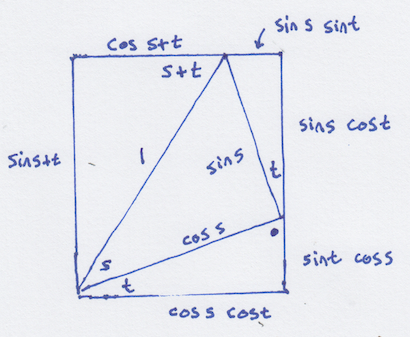
\includegraphics [scale=0.6] {S2.png} \end{center}

For angle $t$, the sine is $\sin t \cos s$ since when it is divided by the hypotenuse $\cos s$ it gives the desired result.  You can just read off both addition formulas.
\[ \sin s + t = \sin s \cos t + \sin t \cos s \]
\[ \cos s + t = \cos s \cos t - \sin s \sin t \]

To get the subtraction formulas, use the fact that $- \sin t = \sin - t$ but $\cos t = \cos -t$.  Cosine is an even function, and sine an odd one.  For example
\[ \cos s - t = \cos s \cos (-t) - \sin s \sin (-t) \]
\[ = \cos s \cos t + \sin s \sin t \]
This is the one to remember if you need to do so.  It's easy to check since if $s = t$, the left-hand side is the cosine of zero which is $1$, and the right-hand side is our favorite trig identity.

$\square$

I don't usually write parentheses in these formulas, but for the rest of the chapter we're going to be doing some algebra and I think it'll make things less confusing.

\subsection*{proof from Ptolemy}

We recall Ptolemy's theorem:  for a cyclic quadrilateral (all 4 vertices on one circle), the sum of the products of the opposing sides is equal to the product of the diagonals.
\begin{center} \includegraphics [scale=0.5] {pt1.png} \end{center}

Draw the diagram corresponding to a special case, where one of the diagonals is a diameter of the circle, scaled so that the length of the diameter is $1$ (below).

Then, draw any two points on the circle (split by the diameter), which give two right triangles, by Thales theorem.  With this scaling, the dotted line is exactly $\sin (\theta + \phi)$, since the factor of $2R$ is equal to $1$.
\begin{center} 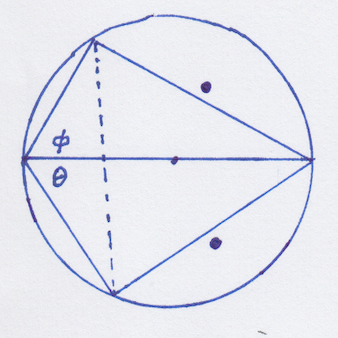
\includegraphics [scale=1.0] {S8.png} \end{center}
So the product of the diagonals is exactly the same.

What about the sides?  Rather than label them, I've just marked two sides with dots, these correspond to the sines of the two angles.  We can read the formula for the sum of sines off the diagram, it is:
\[ \sin (\theta + \phi) = \sin \theta \cos \phi + \sin \phi \cos \theta \]

$\square$

Notice that both products on the right-hand side are the sides of the quadrilateral so they add in the formula.

The other two formulas which have a minus sign will be set up differently, with the dotted line and diagonal as sides of the quadrilateral.

In the next figure, the dotted line is $\sin \theta - \phi$.  It is multiplied by the diameter, which is $1$, as before.
\begin{center} 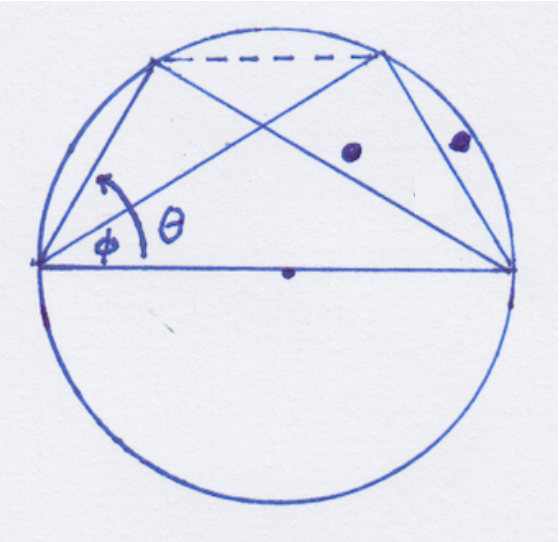
\includegraphics [scale=0.6] {S9b.png} \end{center}
The product of the other pair of sides of the quadrilateral is $\sin \phi \cos \theta$.  The product of diagonals is $\sin \theta \cos \phi$, giving
\[ \sin \phi \cos \theta + \sin (\theta - \phi) = \sin \theta \cos \phi \]
Rearranged
\[ \sin (\theta - \phi) = \sin \theta \cos \phi - \sin \phi \cos \theta \]

$\square$

See if you can show that the other angle that has the dotted line as its chord in the figure above, is also equal to $\theta - \phi$.

It is pretty straightforward to set these up and play around with the angles and sides to massage them into the formulas (since we already know the answer).  

There is one more little trick.  So far the dotted line has been the sine of an angle, but now we need it to be the cosine of an angle.  We obtain that by the following manipulation.  If $s$ and $t$ are complementary angles then
\[ \sin s = \cos t = \cos (90 - s) \]

Next, we use a diagram where the dotted line is a diagonal of the quadrilateral.  That will lead to a formula in which the other terms are summed, which is the formula for the difference of cosines.

Let's see.
\begin{center} 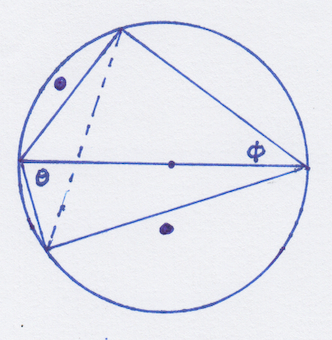
\includegraphics [scale=1.0] {S11.png} \end{center}
The dotted line is the sine of $\theta$ plus something, namely, the complement of $\phi$, so that's $\sin (\theta + 90 - \phi)$.  Remembering what we said about switching to cosine, we take the complement:
\[ \cos \ [ \ 90 - (\theta + 90 - \phi) \ ] \ = \cos (\phi - \theta) \]
The terms from the sides are easy
\[ \cos \theta \cos \phi + \sin \theta \sin \phi = \cos (\phi - \theta) \]
Rearranged:
\[ \cos (\phi - \theta) = \cos \theta \cos \phi + \sin \theta \sin \phi \]

The left-hand side is symmetrical in $\theta$ and $\phi$, but the other side is not.  However, notice that we could just as easily have written $\sin (\phi + 90 - \theta)$ at the beginning.  Then we would have $\cos (\theta - \phi)$ now.  So
\[ \cos (\phi - \theta) = \cos \theta - \phi = \cos \theta \cos \phi + \sin \theta \sin \phi  \]
and that's right!  Cosine is an even function:  
\[ f(x) = f(-x) \ \ \ \text{and} \ \ \  -(\theta - \phi) = \phi - \theta \]

$\square$

There is one more.  This formula has a minus sign in it so it must have the dotted line as one of the sides of the quadrilateral.
\begin{center} 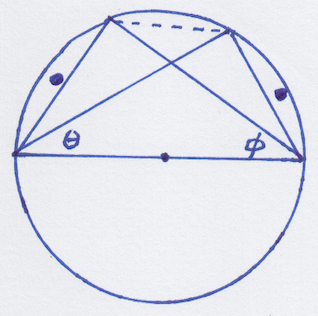
\includegraphics [scale=1.0] {S10.png} \end{center}

The product of diagonals is $\cos \theta \cos \phi$ and one pair of sides is $\sin \theta \sin \phi$.  Since the formula is 
\[ \sin \theta \sin \phi + \cos (\theta + \phi) = \cos \theta \cos \phi \]
\[ \cos (\theta + \phi) = \cos \theta \cos \phi - \sin \theta \sin \phi \]
somehow, the dotted line \emph{must} be $\cos (\theta + \phi$).  I leave the last step to you.  

Don't forget the square at the end of the proof.

\end{document}